\chapter{Evaluation}

\section{Datasets Used}
\label{sec:gliederung}

To evaluate the developed algorithm, two datasets were used:

\begin{itemize}
  \item The Crop Row Benchmark Dataset (CRBD)  \cite{CRBD} is a collection of images featuring various types of crops that can be used to evaluate crop row detection methods. The dataset includes pictures of crops such as maize, celery, potato, onion, sunflower, and soybeans, with varying levels of weeds and shadows. Some images also contain elements such as grass, sky, or roads. The images were taken at different angles and captured using a Panasonic LUMIX DMC-F2 digital camera in the spring of 2014 in the Croatian region of Slovenia. The dataset has a total of 281 images, including 47 images of straight crop rows, which are the main focus of interest of this project.

  
  \item Caterra's own dataset, taken with its front camera intel realsense d435i. It was used to evaluate the algorithm on time-related frames. For this data set that contains no ground truth, a simple visual validation was conducted. 
\end{itemize}

It is important to point out that further evaluations should be conducted on the algorithm, especially to evaluate it on video and later to use it in real time. 
Weather conditions such as rain, snow, and heavy mist were not evaluated as not part of any dataset. 

\section{Results on the Crop Row Benchmark Dataset}
\label{sec:gliederung}

\subsection{Evaluation Method}
\label{sec:gliederung}

To compare the results obtained against the ground truth, two matrices are constructed, one for the ground truth and one for the algorithm developed. In this matrix, the number of rows corresponds to the number of image rows (h), and each row of the matrix has m elements, represented by the horizontal coordinates of m adjacent crop rows detected by the method considered in the v-th image row. 
To compute the accuracy, we use the CRDA formula defined in \cite{8730214} as:


\begin{equation}
CRDA = \frac{1}{m*(h-v_0)} \sum_{v=v_{0}}^{h-1} \sum_{i=1}^{m} s(u_{v,i}^{\ast}, u_{v,i}, d_{v}^{\ast})
 	\label{eq:my_equation}
\end{equation}

with : 
\begin{equation}
s(u^{\ast}, u, d^{\ast}) = max\left(1-\left(\frac{u^{\ast}-u}{\sigma d}\right)^{2}, 0\right)
 	\label{eq:my_equation}
\end{equation}

\newenvironment{conditions*}
  {\par\vspace{\abovedisplayskip}\noindent
   \tabularx{\columnwidth}{>{$}l<{$} @{}>{${}}c<{{}$}@{} >{\raggedright\arraybackslash}X}}
  {\endtabularx\par\vspace{\belowdisplayskip}}

\begin{eqexpl}[5mm]
\item{$m$}{number of crops to be detected}
\item{$v_0$}first line where evaluation starts (could be bushy with undefined crop position on top of image)
\item{$h$}height of the image
\item{$u^{\ast}$}ground truth on line v
\item{$u$}{personal results on line v}
\item{$\sigma$}user defined parameter that is set based on the accuracy needed: in the following evaluation, it is set to 0.3, which means that the matching score is greater than zero only if the horizontal distance between a detected crop row and the corresponding ground truth curve is less than 30\% of the distance between adjacent crop rows
\item{$d^{\ast}$}distance between crops in ground truth
\end{eqexpl}


\subsection{Results}
\label{sec:gliederung}

Our algorithm achieved a median CRDA of 0.816. 
Some examples of detected crop rows and their score are shown in Fig. \ref{pics:resultsdiffcroprow}. %PB HERE
The algorithm presents better results for less bushy crop rows, as when bushes are too present, the Hough transform has many lines to choose from. When weeds are far too present in the center of the crop rows, the algorithm may detect an extra row - this is hopefully not the case if an agricultural robot passes regularly. It is also worth noting that some of the crops from the CRDA images are indistinguishable even from the human eye. \\

Despite the high level of accuracy, the current computational time of the algorithm is too high to be implemented in real-time applications. While the images process using sanely the RANSAC were computed in milliseconds, the average time to process an image using the Hough Transform was 10 seconds. Depending on the accuracy image, this transform can be performed very regularly, which is not practical for real-time applications. As a future work,
it would be important to optimize the algorithm's computational time, to enhance the possibility of using it in real-time applications.

\begin{table}[h]
\begin{center}
 \label{tab:tabnefz}
 \begin{tabular}{|l|l|l|l|l}
 \hline
 Datasets & Mean & Median \\ \hline \hline
 All Crop Rows & 0.773 & 0.816 \\
 Non bushy crop rows & 0.821 & 0.856  \\
 Bushy crop row & 0.625 & 0.689 \\
 \hline
 \end{tabular}
\end{center}
 \caption{Results on the CRBD}\vspace{1ex}

\end{table}


\begin{figure}[H]
\centering
\begin{subfigure}{0.49\textwidth}
    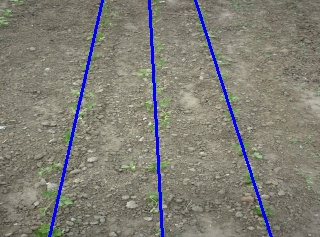
\includegraphics[width=\textwidth]{Report/images/ransac001.jpg}
    \caption{CRDA score of 0.952}
    \label{fig:first}
\end{subfigure}
\begin{subfigure}{0.49\textwidth}%
    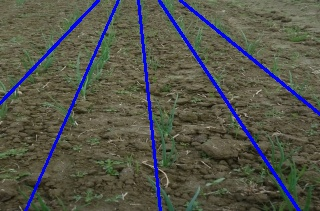
\includegraphics[width=\textwidth]{Report/images/ransac002.jpg}
    \caption{CRDA score of 0.853}
    \label{fig:second}
\end{subfigure}
\begin{subfigure}{0.49\textwidth}%
    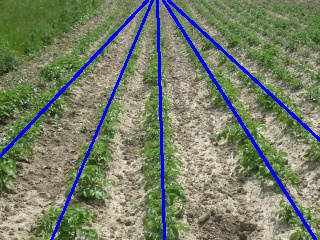
\includegraphics[width=\textwidth]{Report/images/ransac008.jpg}
    \caption{CRDA score of 0.797}
    \label{fig:third}
\end{subfigure}
\begin{subfigure}{0.49\textwidth}%
    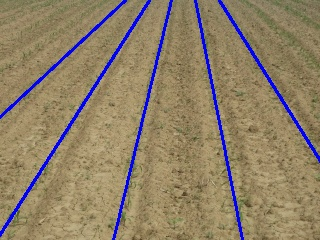
\includegraphics[width=\textwidth]{Report/images/ransac095.jpg}
    \caption{CRDA score of 0.984}
    \label{fig:third}
\end{subfigure}
\caption{Results of the algorithm on different types of crop rows}
\label{pics:resultsdiffcroprow}
\end{figure}

\section{Results on Caterra's dataset}

The Rosbag was captured using the rover's front camera, a realsense d435i.  
The Rosbag contained 776 images of the rover advancing in the field. For visualization, the annotated video can be seen here : \url{https://youtu.be/yA1oaAT4Wgg}.

Depending on the accuracy needed, the number of frames before recalculating the Hough transform and the vanishing point varies. For the visualized video, we have chosen $K=5$.

Crops are detected accurately most of the time, and when an error occurs, it is quickly corrected by the algorithm when this one recalculates the hough transform.

\begin{figure}
\centering
\begin{subfigure}{0.49\textwidth}
    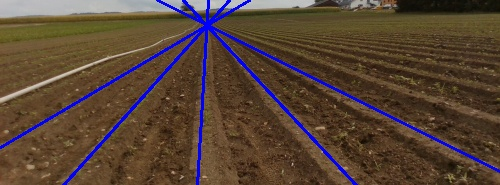
\includegraphics[width=\textwidth]{Report/images/rgb000.jpg}
    \label{fig:first}
\end{subfigure}
\begin{subfigure}{0.49\textwidth}
    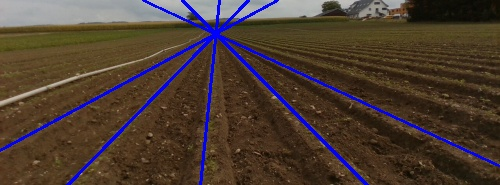
\includegraphics[width=\textwidth]{Report/images/rgb200.jpg}
    \label{fig:first}
\end{subfigure}
\begin{subfigure}{0.49\textwidth}
    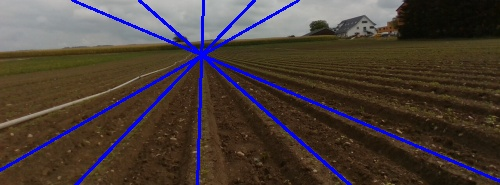
\includegraphics[width=\textwidth]{Report/images/rgb400.jpg}
    \label{fig:first}
\end{subfigure}
\begin{subfigure}{0.49\textwidth}
    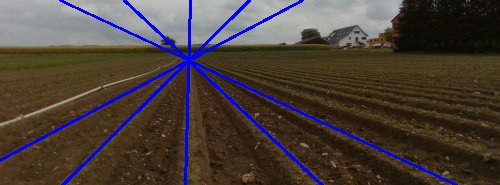
\includegraphics[width=\textwidth]{Report/images/rgb600.jpg}
    \label{fig:first}
\end{subfigure}
\caption{Annotated frames 0, 200, 400, and 600 of the dataset}
\end{figure}
